\xiti
\begin{xiaotis}

\xiaoti{已知长方体形的铜块长、宽、高分别是 2 cm、4 cm、8 cm,将它熔化后铸成一个正方体形的铜块。
    求铸成的铜块的棱长(不计损耗)。
}

\xiaoti{一个长方体的长、宽、高的比为 $1:2:3$,对角线长是 $2\sqrt{14}$ cm。 求它的体积。}

\xiaoti{如图,将正四棱柱底面的边三等分,过三等分点用平行于侧棱的平面截去四个三棱柱,得到一个八棱柱。
    这个八棱柱的体积是原四棱柱体积的几分之几?
}

\begin{figure}[htbp]
    \centering
    \begin{minipage}[b]{7cm}
        \centering
        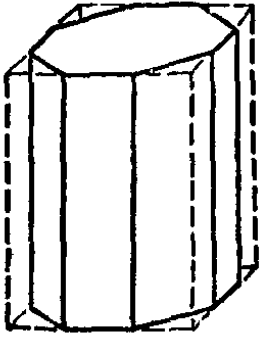
\includegraphics[width=3cm]{../pic/ltjh-ch2-xiti12-03.png}
        \caption*{(第 3 题)}
    \end{minipage}
    \qquad
    \begin{minipage}[b]{7cm}
        \centering
        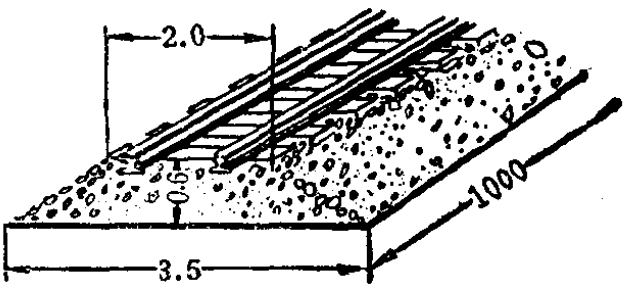
\includegraphics[width=7cm]{../pic/ltjh-ch2-xiti12-06.png}
        \caption*{(第 6 题)}
    \end{minipage}
\end{figure}

\xiaoti{将一个正三棱柱形的木块,旋成与它等高并且尽可能大的圆柱形,旋去的部分是三棱柱体积的几分之几?}

\xiaoti{求证:经过长方体相对的两个面的中心的任意平面,把长方体分成体积相等的两个柱体。}

\xiaoti{要修建铁路,路基如图(单位:m),修建每 1 公里铁路需要碎石多少方($\lfm$)?}

\xiaoti{在一块平地上,计划修建一条水渠,渠道长 1.5 km,渠道断面是梯形,
    梯形两底分别是 1.8 m、0.8 m,高是 0.6 m。如果每人一天挖土 $2\;\lfm$,
    完成这条渠道需要多少个工?
}

\xiaoti{拟修建堤坝 1.5 公里。 坝的断面是梯形,上底宽 4 m,迎水坡宽 20 m,
    迎水坡、背水坡与水平面分别成 $30^\circ$、 $45^\circ$ 的二面角。
    一台推土机每天推土 $80 \; \lfm$,用 5 台推土机几天完成?
}

\xiaoti{我国万吨水压机上,有四根圆筒形钢柱,高 18 m,内径 0.4 m,外径 1 m。
    求这四根钢柱的重量(钢的比重是 $7.8 \; \kmlflm$)。
}

\xiaoti{求证:底面是梯形的直棱柱的体积,等于两个平行侧面面积的和与这两个侧面间距离的积的一半。}

\xiaoti{已知正六棱柱较长的一条对角线长是 13 cm,侧面积是 $180\;\pflm$。 求这个棱柱的体积。}

\xiaoti{一根圆木料,长 3.0 m,直径 0.8 m,距圆木的轴 0.2 m 且平行于轴锯去一片,求剩余木料有多少立方米。}

\end{xiaotis}

